
\chapter{La Función Gamma}\label{aped.A}
\begin{defn} Dado $x\in\mathds{R}^+$ definimos la función gamma\cite[sec. 1.2]{libro_esfarm} como
	$$
	\Gamma(x) := \int_{0}^{\infty} t^{x-1}e^{-t}dt		
	$$
\end{defn}
\begin{prop}Se verifican las siguientes formulas:
	\begin{gather}
	\begin{aligned}
	&\int_{0}^{\infty}  t^{x-1}e^{-at^b}dt = b^{-1}a^{-x/b}\Gamma(x/b)  , x,a,b \in \mathds{R}^+ \\
	&\int_{0}^{1} |\ln{t}|^{x-1}dt = \Gamma(x),   x \in \mathds{R}^+  \\
	&\Gamma(x+1) = x \Gamma(x) ,		x\in \mathds{R}^+ \\
	&\Gamma^{(k)}(x) = \int_{0}^{\infty} (\ln{t})^k t^{x-1} e^{-t} dt,   k\in\mathds{N}_0,x\in\mathds{R}^+ \\
	\end{aligned}
	\end{gather}
\end{prop}
\begin{rem}
	$\Gamma(1)=1$ y de la tercera fórmula se deduce que $\Gamma(n+1)=n!, n\in\mathds{N}_0$. Es decir, la función $\Gamma$ extiende el operador factorial de los números naturales a los reales positivos.
\end{rem}
\begin{lem} 
	$$
	\Gamma(\frac{1}{2}) = 	\sqrt{\pi}
	$$
	$$
	\Gamma(n+\frac{1}{2})=\frac{(2n)!}{2^{2n}n!} \sqrt{\pi}
	$$
\end{lem}
\begin{defn}Sea $x\in\mathds{R}$ y $n\in\mathds{N}$, el símbolo de Pochhammer se define como
	$$
	(x)_0 = 1, (x)_n=x(x+1)(x+2)...(x+n-1)
	$$
\end{defn}
\begin{prop} Sea $x\in\mathds{R}^+$ entonces
	$$
	(x)_n = \frac{\Gamma(x+n)}{\Gamma(x)}
	$$
\end{prop}
\chapter{Resultados básicos de la esfera.}\label{aped.B}
En esta sección presentaremos algunos resultados referentes a la esfera que nos serán de utilidad \cite[sec 1.3]{libro_esfarm}.
\bigskip

En $\mathds{R}^d$ usaremos la base canónica 

$$ e_1 =(1,0,0,...,0)^T ,...,e_d=(0,...,0,1)^T $$

Usaremos $dV^d$ para elemento diferencial de volumen y $dS^{d-1}$ para elemento diferencial de superficie de la esfera $\mathds{S}^{d-1}$.

\begin{prop}(Coordenadas polares)
\begin{gather}
\begin{aligned}
x_1 &= r \cos \theta \\
x_2 &= r \sen \theta \\
\end{aligned}
0 \le \theta \le 2\pi, r\le 0
\end{gather}
\end{prop}

\begin{prop}(Coordenadas esféricas)
\begin{gather*}
\begin{aligned}
x_1 &= r \sen \theta \sen \phi\\
x_2 &= r \sen \theta \sen \phi\\
x_3 &= r \cos \theta\\
\end{aligned}
\\
0\le \theta \le \pi,0\le\phi\le2\pi,r>0
\end{gather*} 
\end{prop}
\begin{prop}Para $d \ge 3$ y $\xi \in \mathds{S}^{d-1}$,con $\xi_{(d)} = te_d+\sqrt{1-t^2}\xi_{(d-1)},  t\in[-1,1]$ , se tiene que
	$$
	dS^{d-1}(te_d+\sqrt{1-t^2}\xi_{(d-1)}) = (1-t^2)^{\frac{d-3}{2}}dt  dS^{d-2}(\xi_{(d-1)})
	$$
	Equivalentemente,
	$$
	dS^{d-1} = (1-t^2)^{\frac{d-3}{2}}dt dS^{d-2}
	$$
\end{prop}
\begin{example}Sea d=3 y $\xi$ un punto genérico de la esfera. Usando coordenadas esféricas $$
	\xi_{(3)}=\begin{pmatrix}
	\cos\phi \sen\theta\\
	\sen\phi \sen\theta\\
	\cos\theta\\
	\end{pmatrix}
	0 \le \phi \le 2\pi , 0 \le \theta \le \pi
	$$
	Sea $t=\cos\theta$ entonces
	$$
	\xi_{(2)} = \begin{pmatrix}
	\cos\phi\\
	\sen\phi\\
	0\\
	\end{pmatrix}
	$$
	Por tanto,$ \xi_{(3)} = te_3 + \sqrt{1-t^2} \xi_{(2)}$ y $dS^1 = d\phi , dS^2 = dtd\phi$
	
\end{example}
Podemos usar la anterior proposición para el cálculo del área de la superficie de la esfera.
\begin{prop}Se verifica que
	$$
	|\mathds{S}^{d-1}| = \int_{\mathds{S}^{d-1}} dS^{d-1} = \frac{2\pi^\frac{d}{2}}{\Gamma(\frac{d}{2})}
	$$
\end{prop} 

\begin{prop}
	Sea $A\in\mathds{R}^{d\times d}$ ortogonal entonces
	$$ dS^{d-1}(A\xi) =  dS^{d-1}(\xi)$$
	$$ dV^{d}(A\xi) =  dV^{d}(\xi)$$
\end{prop}

Llamamos $C(S^{d-1})$ al espacio de funciones continuas sobre  $S^{d-1}$. Este espacio es un espacio de Banach con la norma $ ||f||_\infty = \sup \{ |f(\xi) : \xi\in \mathds{S}^{d-1}\}$. Llamaremos $L^2(S^{d-1})$ al espacio de funciones con cuadrado integrable en $S^{d-1}$. Dicho espacio es un espacio de Hilbert con el producto escalar$$ (f,g) = \int_{S^{d-1}} f\overline{g} dS^{d-1}
$$
Consideramos el espacio $C(S^{d-1})$ con la norma inducida por el producto escalar de $L^2(S^{d-1})$. Este espacio no es completo. Además, el cierre de $C(S^{d-1})$ respecto a dicha norma es $L^2(S^{d-1})$. Es decir, dado una función $f\in L^2(S^{d-1})$ existe una sucesión $\{f_n\} \subset C(S^{d-1})$ tal que ${f_n}\to f$

\begin{prop}Sean $\Omega_\delta = \{x\in\mathds{R}^d : |x|\in[1-\delta,1+\delta]\}$ y $f^*(x)= f(\frac{x}{|x|}),x\in\Omega_\delta$ y $k\in\mathds{N}$.Entonces $f$ es k veces diferenciable en $S^{d-1}$ cuando $f^*$ lo es.  
\end{prop}
\begin{defn}Definimos $C^k(S^{d-1}), k\in\mathds{N}\cup0$ como el espacio de funciones k veces diferenciables en $S^{d-1}$
\end{defn}
\begin{prop}$C^k(S^{d-1})$ es un espacio de Banach con la norma 
	$$
	||f||_{C^k(S^{d-1})} = ||f^*||_{C^k(\Sigma_\delta)}
	$$
\end{prop}
\begin{rem}Usaremos $||f||_\infty = ||f||_{C(S^{d-1})}$
	
\end{rem}
\chapter{Polinomios de Legendre}\label{aped.C}
\section{Fórmulas de Representación}
\subsection{Fórmula de Rodrigues}
\begin{thm}
	$$P_{n,d}(t) = (-1)^n \frac{\Gamma(\frac{d-1}{2}) }{2^n\Gamma(n+\frac{d-1}{2})}(1-t^2)^{\frac{3-d}{2}}(\frac{d}{dt})^n (1-t^2)^{n+\frac{d-3}{2}}, \quad d\ge2
	$$
\end{thm}
\begin{rem}\label{cte_Rod}
	A la constante $R_{n,d} = \frac{\Gamma(\frac{d-1}{2})}{2^n\Gamma(n+\frac{d-1}{2})}$ se le llama constante de Rodrigues
\end{rem}
\begin{rem}
	Estos polinomios verifican $P_{n,d}(1)=1$ y $\int_{-1}^{1} P_{n,d}(t)P_{m,d}(t)(1-t^2) dt= 0$ para $m\le n$
\end{rem}
\begin{example}
	\begin{itemize}
		\item Si d = 2, $$P_{n,2}(t) = (-1)^n \frac{2^n n!} {(2n)!}(1-t^2)^{\frac{1}{2}}(\frac{d}{dt})^n (1-t^2)^{n-\frac{1}{2}}, \quad n\in \mathds{N}_0$$ Una forma reducida se obtiene usando el polinomio de Chebyshev obteniendo que $P_{n,2}(t) = \cos(n \quad \arccos{t}), t\in[-1,1]$
		\item Si d=3, $$P_{n,3}(t) = \frac{1} {2^n n!}(\frac{d}{dt})^n (t^2-1)^{n}, \quad n\in \mathds{N}_0$$
	\end{itemize}
\end{example}
\subsection{Fórmulas de Representación Integral.}
\begin{thm}Sea $n\in\mathds{N}_0$ y $d\ge3$, $$ 
	P_{n,d}(t) = \frac{|\mathds{S}^{d-3}|}{|\mathds{S}^{d-2}|}\int_{-1}^{1}[t+i(1-t^2)^{\frac{1}{2}}s]^n(1-s^2)^{\frac{d-4}{2}} ds, \quad t\in[-1,1]
	$$
\end{thm}
\begin{rem}Como consecuencia de la fórmula anterior se tiene que $P_{n,d}(-t) = (-1)^n P_{n,d}(t), t\in[-1,1]$, es decir $P_{n,d}(t)$ tiene la misma paridad que $n$.
\end{rem}
%Podemos obtener otra fórmula de representación integral, usando funciones trigonométricas mediante el cambio de variable $s = tanh(u), u\in\mathds{R}$
%\begin{thm}Sea $n\in\mathds{N}_0$ y $d\ge3$, $$
%		P_{n,d}(t) = \frac{|\mathds{S}^{d-3}|}{|\mathds{S}^{d-2}|}\int_{-1}^{1}\frac{(1-s^2)^{\frac{d-4}{2}}}{[t\pm i(1-t^2)^{\frac{1}{2}}s]^{n+d-2}} ds, \quad t\in(0,1]
%	$$
%\end{thm}
\section{Propiedades}
\begin{prop}
Si $f\in C^n([-1,1])$ entonces 
$$
\int_{-1}^{1} f(t)P_{n,d}(t)(1-t^2)^{\frac{d-3}{2}} dt = R_{n,d}\int_{-1}^{1} f^{(n)}(t)(1-t^2)^{n+\frac{d-3}{2}} dt
$$
siendo $R_{n,d}$ la constante de Rodrigues \hyperref[]{(Nota \ref{cte_Rod})}
\end{prop}
\begin{prop}(Norma)
	$$ \int_{-1}^{1} \left[P_{n,d}(t)\right]^2(1-t^2)^{\frac{d-3}{2}} dt = \frac{\sqrt{\pi} \Gamma(\frac{d-1}{2})}{\frac{(2n+d-2)(n+d-3)!}{n!(d-2!)}\Gamma(\frac{d}{2})}$$
\end{prop}
\begin{prop}(Ecuación diferencial)
	$$(1-t^2)P_{n,d}''(t) - (d-1)tP_{n,d}(t)'+n(n+d-2)P_{n,d}(t) = 0 $$
\end{prop}
\begin{prop}$P_{n,d}(t)$ tiene n raíces distintas en (-1,1)
\end{prop}
\begin{prop}Los polinomios de Legendre satisfacen la siguiente relación de recurrencia
	\begin{gather*}
		P_{n,d}(t) = \frac{2n+d-4}{n+d-3}t	P_{n-1,d}(t) - \frac{n-1}{n+d-3}P_{n-2,d}(t), \qquad n\ge 2, d\ge2 \\
		P_{0,d}(t) = 1 , 	P_{1,d}(t) = t 
	\end{gather*}
\end{prop}
\begin{prop}
	\begin{gather*}
	(1-t^2)P'_{n,d}(t) = n[P_{n-1,d}(t)-tP_{n,d}(t)], \quad n \ge 1,d \ge 2, t \in [-1,1]
	\end{gather*}
\end{prop}
\begin{prop}Para $d\ge 2$
$$\sum_{n=0}^{\infty} \frac{(2n+d-2)(n+d-3)!}{n!(d-2!)}r^nP_{n,d}(t) = \frac{1-r^2}{(1+r^2-2rt)^\frac{d}{2}},\quad |r| < 1, t\in[-1,1] 
$$
\end{prop}
\begin{prop}
	\begin{gather*}
	P_{n,d}(0) = \frac{|\mathds{S}^{d-3}|}{|\mathds{S}^{d-2}|}\int_{-1}^{1} i^n s^n(1-s^2)^{\frac{d-4}{2}}ds \\
	P_{n,d}(-1) = (-1)^n
	\end{gather*}
\end{prop}
\begin{prop}
	$$
	|P_{n,d}(t)| < \frac{\Gamma(\frac{d-1}{2})}{\sqrt{\pi}}\left[\frac{4}{n(1-t^2)}\right]^{\frac{d-2}{2}},\quad n\in\mathds{N}_0,d\ge2,t\in(-1,1)$$
\end{prop}

\chapter{Polinomios de Gegenbauer}\label{aped.D}
En esta sección estudiaremos los polinomios de Gegenbauer \cite[sec. 2.9]{libro_esfarm}
\begin{defn}Sean $v\ge 0,n\in\mathds{N}_0$ se define el polinomio de Gegenbauer de grado $n$ e índice $v$, como:
	$$C_{n,v}(t) = \binom{n+2v-1}{n}\frac{\Gamma(v+\frac{1}{2})}{\sqrt{\pi}\Gamma(v)}\int_{-1}^{1}\left[t+i(1-t^2)^{1/2}s\right]^n (1-s^2)^{v-1} ds$$ 
\end{defn}
Los polinomios de Gegenbauer coinciden con los polinomios de Legendre salvo una constante de normalización.
\begin{prop}\label{geb_rel}Se verifica la siguiente relación
	$$C_{n,\frac{d-2}{2}}(t) = \begin{pmatrix}
	n+d-3 \\
	d
	\end{pmatrix} P_{n,d}(t)
	$$
\end{prop}
\begin{prop}(Función generatriz)$$
	\sum_{n=0}^{\infty} C_{n,v}(t) = \frac{1}{(1+r^2-2rt)^v}, \qquad |r|<1, t\in[-1,1]$$
\end{prop}
%ec. diferencial%
\begin{prop}\label{Ggdif}(Ecuación diferencial, \cite[sec 4.7]{libro_gegen})
	$$
	(1-x^2)C_{n,v}''(x)-(2v+1)xC_{n,v}'+n(n+2v)C_{n,v} = 0
	$$
\end{prop}
\begin{prop}\label{propGg} Se verifican las siguientes igualdades:
	\begin{enumerate}[(i)]
	\item $\frac{d}{dx} C_{n,v}(x) = 2v C_{n-1,v+1}(x)$
	\item $nC_{n,v}(x) = x\frac{d}{dx} C_{n,v}(x) - \frac{d}{dx} C_{n-1,v}(x)$
	\item $(n+2v) C_{n,v}(x)  = \frac{d}{dx}C_{n-1,v}(x)-x \frac{x}{dx}C_{n,v}(x) \quad n\ge 0$
	\item $\begin{aligned}
		\frac{d}{dx} \left[C_{n+1,v}(x) - C_{n-1,v}(x)\right]  &= 2(n+v)C_{n,v}(x)\\ &= 2v \left[C_{n,v+1}(x) - C_{n-2,v+1}(x)\right] \quad n\ge 1
	\end{aligned}$        	
\end{enumerate}
\end{prop}
\chapter{Funciones de Legendre Asociadas}\label{aped.E}

Las funciones asociadas de Legendre \cite[sec. 2.10]{libro_esfarm} nos permiten construir armónicos esféricos a partir de otros de menor dimensión.
\begin{defn}Sea $d\ge3$ y $n,j \in \mathds{N}_0$ se define la función asociada de Legendre de grado n y orden j en dimensión d, como
	$$
	P_{n,d,j}(t) = \frac{|\mathds{S}^{d-3}|}{|\mathds{S}^{d-2}|}i^{-j} \int_{-1}^{1}\left[t+i(1-t^2)^{1/2}s\right]^n P_{j,d-1}(s)(1-s^2)^{\frac{d-4}{2}}, \quad t\in[-1,1]
	$$
\end{defn}
\begin{rem}Si $j=0, P_{n,d,0}(t)=P_{n,d}(t)$
\end{rem}
%Las funciones asociadas de Legendre nos permiten generar "sistemas" de esféricos armónicos en la esfera.
\begin{prop}Sea $d\le3$ y $0\le j \le n$ 
	$$	P_{n,d,j}(t) = \frac{n!\Gamma(\frac{d-1}{2})}{2^j(n-j)!\Gamma(j+\frac{d-1}{2})}(1-t^2)^{1/2} P_{n-j,d+2j}(t), t\in[-1,1]$$
\end{prop}
El siguiente resultado nos proporciona una relación entre las funciones asociadas de Legendre y las derivadas de los polinomios de Legendre.
\begin{prop}Sea $d\le3$ y $0\le j \le n$ 
	$$	P_{n,d,j}(t) = \frac{(n+d-3)!}{(n+j+d-3)!}(1-t^2)^{1/2} P^{(j)}_{n,d}(t), t\in[-1,1]$$
\end{prop}
\begin{prop}
	\begin{gather*}
	\int_{-1}^{1} P_{m,d,j}(t)P_{n,d,j}(t)(1-t^2)^{\frac{d-3}{2}} dt = 0, \qquad m \neq n
	\end{gather*}
\end{prop}
\begin{prop} Las funciones $\tilde{P}_{n,d,j}$ definidas como
	\begin{gather*}
	\tilde{P}_{n,d,j}(t) = \frac{[(2n+d-2)(n-j)!(n+d+j-3)!]^{1/2}}{2^{\frac{d-2}{2}n!\Gamma(\frac{d-1}{2})}}P_{n,d,j}(t), \quad t\in[-1,1]
	\end{gather*}
	están normalizadas, es decir $\int_{-1}^{1} [	\tilde{P}_{n,d,j}]^2(1-t^2)^\frac{d-3}{2} dt = 1$
\end{prop}
\begin{rem}\label{note:fun_leg}Las funciones $	\tilde{P}_{n,d,j}$ pueden ser escritas en función de las derivadas de los polinomios de Legendre 
	\begin{gather*}
	\tilde{P}_{n,d,j}(t) =\frac{(n+d-3)!}{n!\Gamma(\frac{d-1}{2})} \frac{[(2n+d-2)(n-j)!]^{1/2}}{2^{d-2}(n+d+j-3)!}(1-t^2)^{j/2}P^{(j)}_{n,d}(t), \quad t\in[-1,1]
	\end{gather*}
\end{rem}
\chapter{El problema de clasificación}\label{aped.F}
El problema de clasificación consiste en predecir la clase a la que pertenece una instancia basándonos en una serie de características disponibles. Es un tipo de aprendizaje supervisado, es decir, se conoce de antemano la clases a las que pertenecen los ejemplos usados para construir el clasificador.
%meter grafikito%
El proceso de clasificación consta de las siguientes etapas:

\begin{enumerate}
	\item \textbf{Construir el clasificador}. A partir de un conjunto de ejemplos ya clasificados. El modelo resultante establece 
	\item \textbf{Validación}. Se usa un conjunto distinto al de entrenamiento ya clasificado. Para cada instancia de este conjunto se compara el valor devuelto con el valor real.
\end{enumerate}

Una de las técnicas para realizar la evaluación del modelo es la conocida como validación cruzada. Esta técnica consiste en dividir el conjunto de entrenamiento en k partes, usando k-1 partes para construir el clasificador y usar la restante para validar. Este proceso se repite durante k iteraciones de forma que cada parte es usada como conjunto de prueba. Finalmente, se ponderan los resultados de cada iteración para obtener el resultado final.
\begin{figure}
	\centering
	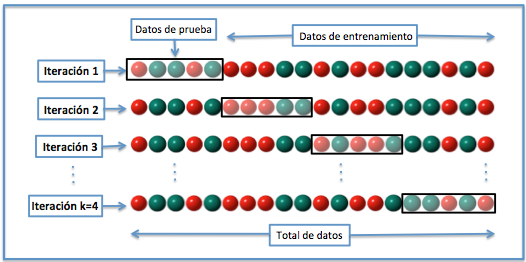
\includegraphics[scale=0.45]{img/K-fold_cross_validation.jpg}
	\caption{Ejemplo validación cruzada.}
\end{figure}
%referencia https://es.wikipedia.org/wiki/Validaci%C3%B3n_cruzada#/media/File:K-fold_cross_validation.jpg
